% lin-rw.tex

\documentclass{standalone}
% newcommands.tex

\newcommand{\enq}{\texttt{enq}}
\newcommand{\deq}{\texttt{deq}}
\newcommand{\pput}{\texttt{PUT}}
\newcommand{\get}{\texttt{GET}}
\newcommand{\vs}{\texttt{vis}}
\newcommand{\so}{\texttt{so}}
\newcommand{\arb}{\texttt{ar}}
\newcommand{\rf}{\texttt{rf}}

% example
\newcommand{\po}[2]{\draw [->, thick] (#1) to node[above] {\Large{\so}} (#2);}
\newcommand{\pva}[2]{\draw [->, thick] (#1) to node[above] {$\Large{\so},\Large{\vs},\Large{\arb}$} (#2);}
\newcommand{\pbva}[2]{\draw [->, thick] (#1) to node[above] {$\Large{\so}$} node[below] {$\Large{\vs},\Large{\arb}$} (#2);}
\newcommand{\pv}[2]{\draw [->, thick] (#1) to node[above] {\Large{\so}} node[below] {\Large{\vs}} (#2);}
\newcommand{\evis}[2]{\draw [->, thick] (#1) to node[above, sloped, near end] {\Large{\vs}} (#2);}
\newcommand{\mvis}[2]{\draw [->, thick] (#1) to node[above, sloped] {\Large{\vs}} (#2);}
\newcommand{\ar}[2]{\draw [->, thick, allow upside down] (#1) to node[above, sloped] {\Large{\arb}} (#2);}
\newcommand{\va}[2]{\draw [->, thick, allow upside down] (#1) to node[above, sloped] {$\Large{\vs},\Large{\arb}$} (#2);}
\newcommand{\vab}[2]{\draw [->, thick, allow upside down] (#1) to node[below, sloped, near end] {$\Large{\vs},\Large{\arb}$} (#2);}
\newcommand{\vae}[2]{\draw [->, thick, allow upside down] (#1) to node[above, sloped, near end] {$\Large{\vs},\Large{\arb}$} (#2);}
\newcommand{\vas}[2]{\draw [->, thick, allow upside down] (#1) to node[sloped, near start, above] {$\Large{\vs},\Large{\arb}$} (#2);}

% serialization
\newcommand{\scc}[2]{\draw [->, very thick] (#1) to (#2);}
\newcommand{\rva}[2]{\draw [->, thick, allow upside down] (#1) to node[above, sloped] {$\Large{\rf},\Large{\vs},\Large{\arb}$} (#2);}
\newcommand{\rvb}[2]{\draw [->, thick, allow upside down] (#1) to node[below, sloped] {$\Large{\rf},\Large{\vs},\Large{\arb}$} (#2);}

\newcommand{\rwevent}{{\sf R\&W}}

\usepackage{tikz}
\usetikzlibrary{calc, shapes, positioning, arrows.meta, decorations.pathmorphing}

\begin{document}
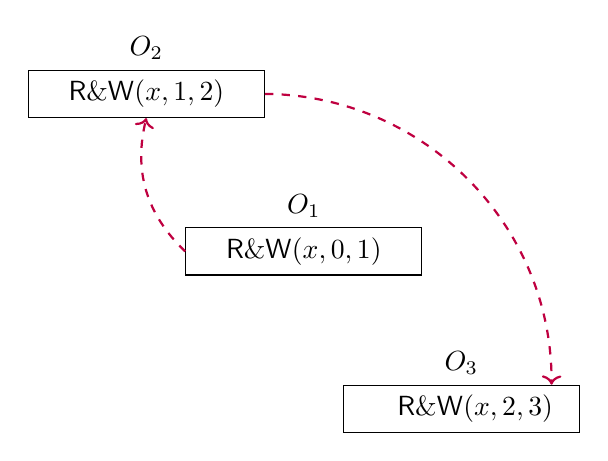
\begin{tikzpicture}[
  so/.style = {->, thick},
	start/.style = {blue, dashed, thick},
	commit/.style = {brown, dotted, very thick},
  txn/.style = {draw, inner sep = 2pt,
	  minimum height = 0.6cm, minimum width = 3.0cm}]

  \node[txn, label = above : $O_{2}$] (t1)
    {$\quad\rwevent(x, 1, 2)\quad$};
	\startcommittime{t1}{0.50cm}{0.50cm}
  \tsorder{t1}{0.80cm}{182}{185} % 1, 4

  \node[txn, label = above : $O_{1}$] (t2)
		at ($(t1) + (2.00cm, -2.00cm)$)
    {$\quad\rwevent(x, 0, 1)\quad$} ;
	\startcommittime{t2}{0.50cm}{0.50cm}
  \tsorder{t2}{0.80cm}{184}{187} % 3, 6

  \node[txn, label = above : $O_{3}$] (t3)
		at ($(t2) + (2.00cm, -2.00cm)$)
    {$\quad\rwevent(x, 2, 3)$};
	\startcommittime{t3}{0.50cm}{0.50cm}
  \tsorder{t3}{0.80cm}{186}{189} % 5, 8

	\draw[->, thick, purple, dashed, bend left] (t2.west) to (t1.south);
	\draw[->, thick, purple, dashed, bend left = 45] (t1.east) to (t3.15);
\end{tikzpicture}
\end{document}